\documentclass[svgnames,11pt]{standalone}
\usepackage[utf8]{inputenc}
\usepackage[T1]{fontenc}
\usepackage{csquotes}
\usepackage[english]{babel}
\usepackage{xcolor}
\usepackage{charter}
\usepackage{amsmath}
\usepackage[np,autolanguage]{numprint}
\usepackage{tikz}
\usetikzlibrary{arrows,automata,calc}
\usetikzlibrary{arrows.meta}
\usetikzlibrary{decorations.pathreplacing}
\usetikzlibrary{backgrounds}
\tikzset{%
  show curve controls/.style={
    postaction={
      decoration={
        show path construction,
        curveto code={
          \draw [blue] 
            (\tikzinputsegmentfirst) -- (\tikzinputsegmentsupporta)
            (\tikzinputsegmentlast) -- (\tikzinputsegmentsupportb);
          \fill [red, opacity=0.5] 
            (\tikzinputsegmentsupporta) circle [radius=.25ex]
            (\tikzinputsegmentsupportb) circle [radius=.25ex];
        }
      },
      decorate
}}}
\tikzstyle{vertex}=[draw,circle,black,inner sep=2pt]
\tikzstyle{edge}=[line width=1.3pt,color=Black]
\tikzstyle{rare}=[fill=black,text=white]
\tikzstyle{medium}=[fill=black!15!white]


\begin{document}
  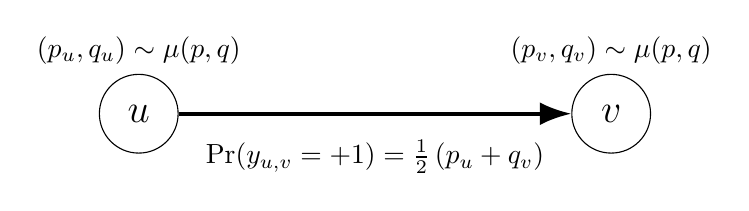
\begin{tikzpicture}[auto,vertex/.append style={minimum width=10mm,font=\Large},
    edge/.append style={-{Latex[length=4mm,width=1.5mm,angle'=40]}},]
    \node[vertex] (u) at (0,0) {$u$};
    \node[anchor=south] (iparams) at (0,0.5) {$(\outqt{p_u}, q_u) \sim \mu(p, q)$};
    \node[vertex,] (v) at (6,0) {$v$};
    \node[anchor=south] (jparams) at (6,0.5) {$(p_v, \inqt{q_v}) \sim \mu(p, q)$};
    \draw[edge,opacity=1] (u) edge node[below,yshift=-2mm] {$\Pr(y_{u,v}=+1) = \frac{1}{2}\left(\outqt{p_u}+\inqt{q_v}\right)$} (v);
  \end{tikzpicture}
\end{document}
